\documentclass[border=4pt]{standalone}
\usepackage{tikz}
\usetikzlibrary{arrows.meta,patterns}
\begin{document}
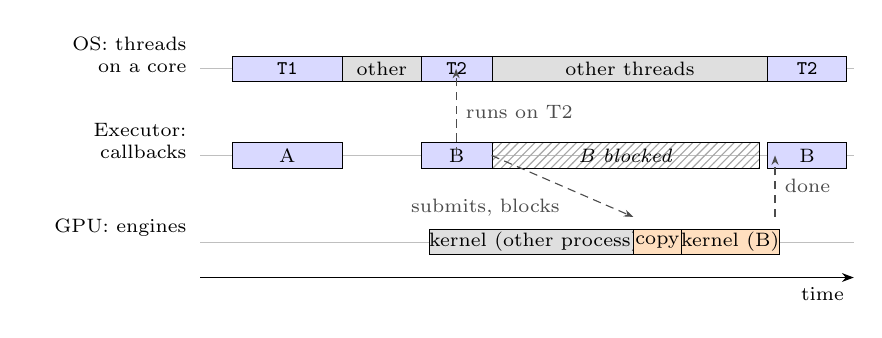
\begin{tikzpicture}[x=1cm,y=1cm,font=\scriptsize,
  seg/.style={draw,minimum height=3.2mm,inner sep=0pt,anchor=west},
  cpu/.style={seg,fill=blue!15}, wait/.style={seg,fill=white,pattern=north east lines,pattern color=gray!70},
  gpu/.style={seg,fill=orange!25}, other/.style={seg,fill=gray!25},
  link/.style={densely dashed,gray!60!black,-{Stealth[length=1.2mm]}}]
\foreach \y/\lab in {2.2/{OS: threads on a core},1.1/{Executor: callbacks},0/{GPU: engines}}{
  \draw[gray!50] (0,\y) -- (8.3,\y);
  \node[anchor=east,align=right,text width=1.9cm] at (-0.05,\y+0.18) {\lab};}
\draw[-{Stealth[length=1.5mm]}] (0,-0.45) -- (8.3,-0.45) node[below left] {time};
\node[cpu,minimum width=1.4cm] at (0.4,2.2) {\texttt{T1}};
\node[other,minimum width=1.0cm] at (1.8,2.2) {other};
\node[cpu,minimum width=0.9cm] at (2.8,2.2) {\texttt{T2}};
\node[other,minimum width=3.5cm] at (3.7,2.2) {other threads};
\node[cpu,minimum width=1.0cm] at (7.2,2.2) {\texttt{T2}};
\node[cpu,minimum width=1.4cm] at (0.4,1.1) {A};
\node[cpu,minimum width=0.9cm] at (2.8,1.1) {B};
\node[wait,minimum width=3.4cm] at (3.7,1.1) {\textit{B blocked}};
\node[cpu,minimum width=1.0cm] at (7.2,1.1) {B};
\node[other,minimum width=2.6cm] at (2.9,0) {kernel (other process)};
\node[gpu,minimum width=0.6cm] at (5.5,0) {copy};
\node[gpu,minimum width=1.2cm] at (6.1,0) {kernel (B)};
\draw[link] (3.25,1.1) -- (3.25,2.2) node[midway,right] {runs on T2};
\draw[link] (3.7,1.1) -- (5.5,0.32) node[pos=.55,below left] {submits, blocks};
\draw[link] (7.3,0.32) -- (7.3,1.1) node[midway,right] {done};
\end{tikzpicture}
\end{document}
